%%%%%%%%%%%%%%%%%%%%%%%%%%%%%%%%%%%%%%%%%%%%%%
\section{Introduction à Buildroot}
%%%%%%%%%%%%%%%%%%%%%%%%%%%%%%%%%%%%%%%%%%%%%%

\begin{frame}{Buildroot}
  \begin{itemize}
  \item Peut compiler une toolchain, un rootfs, un kernel, un bootloader
  \item {\bf Facile à configurer}: menuconfig, xconfig, etc.
  \item {\bf Rapide}: compile un rootfs en quelques minutes
  \item Facile à comprendre: écrit en make, bonne documentation
  \item {\bf Petit}: root filesystem, débute en 2 MB
  \item {\bf 2200+ paquets} pour userspace
  \item {\bf Pleins d'architectures} supportées
  \item {\bf Technologies bien connues}: {\em make} et {\em kconfig}
  \item Neutre
  \item Communauté active, releases régulières
  \item \url{https://buildroot.org}
  \end{itemize}
\end{frame}

\begin{frame}{Buts dans le design}
  \begin{itemize}
  \item Buildroot est designé avec des buts précis:
    \begin{itemize}
    \item Simple à utiliser
    \item Simple à personnaliser
    \item Builds \textbf{reproductibles}
    \item Petit root filesystem
    \item Temps de build relativement rapide
    \item Facile à comprendre
    \end{itemize}
  \item Pas toutes les fonctionnalités possibles supportées
  \item Plus compliqués et avec beaucoup de fonctionnalités : Yocto Project, OpenEmbedded
  \end{itemize}
\end{frame}

\begin{frame}{Buildroot dans l'industrie?}
  \begin{columns}
    \column{0.6\textwidth}
    \begin{itemize}
    \item {\bf Entreprises}
      \begin{itemize}
      \item Google
      \item Barco
      \item Rockwell Collins
      \end{itemize}
    \item {\bf Vendeurs de processors}
      \begin{itemize}
      \item Imagination Technologies
      \item Marvell
      \item Microchip (Atmel)
      \item Analog Devices
      \end{itemize}
    \item {\bf Vendeur de SoM et de cartes}
    \item Beaucoup d'entreprises lors de {\em R\&D} sur des produits
    \item Beaucoup de {\bf hobbyists} des cartes de developpement :
      Raspberry Pi, BeagleBone Black, etc.
  \end{itemize}
  \column{0.4\textwidth}
  \only{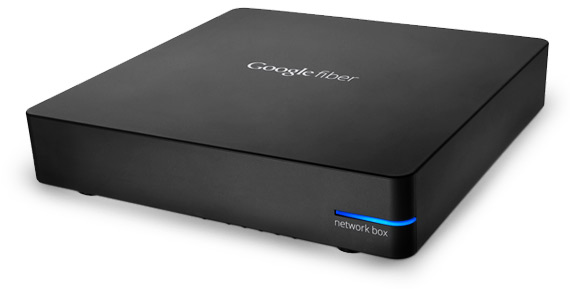
\includegraphics[height=0.25\textheight]{pictures/google-fiber-box.jpg}}\\
  \only{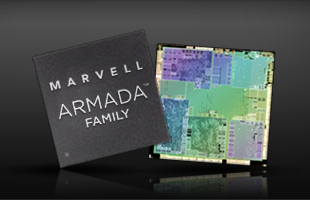
\includegraphics[height=0.25\textheight]{pictures/armada.jpg}}\\
  \only{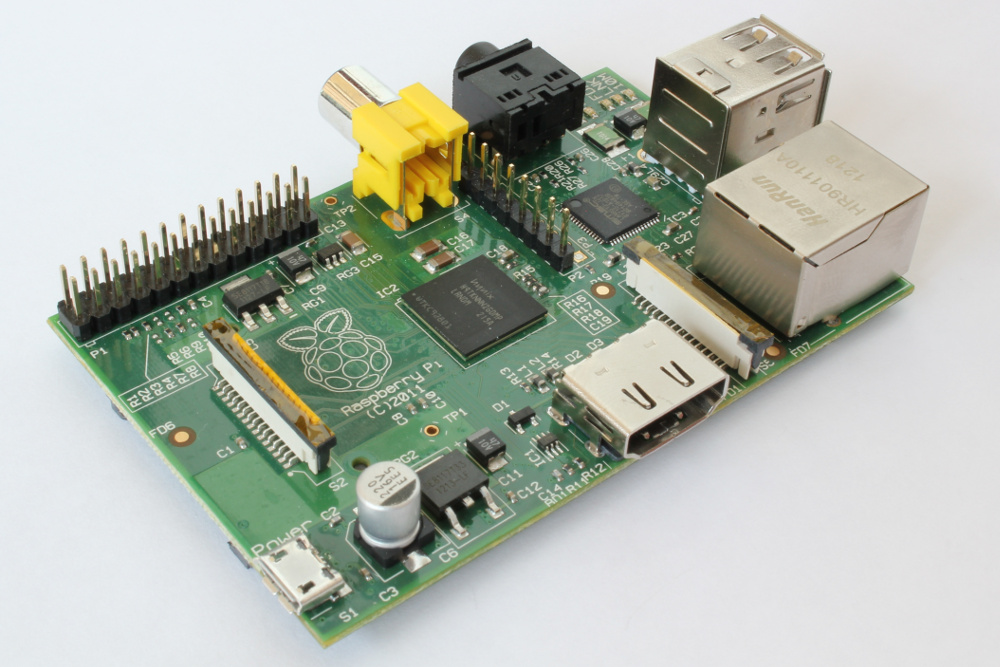
\includegraphics[height=0.25\textheight]{pictures/raspberrypi.jpg}}
  \end{columns}
\end{frame}

\begin{frame}{Buildroot}
  \begin{itemize}
  \item Releases stables tous les 3 mois:
    \begin{itemize}
    \item \code{YYYY.02}, \code{YYYY.05}, \code{YYYY.08},
      \code{YYYY.11}
    \end{itemize}
  \item Archives disponibles pour chaque release stable
    \begin{itemize}
    \item \url{https://buildroot.org/downloads/}
    \end{itemize}
  \item Plus pratique via git
    \begin{itemize}
    \item Visualisation de ses modifications
    \item Simplification des contribution
    \item \code{git clone git://git.busybox.net/buildroot}
    \item Tags git disponible pour chaque release stable
    \end{itemize}
  \item Une {\bf long term support (LTS)} release chaque année
    \begin{itemize}
    \item Maintenue durant 1 an
    \item Fixes de sécurité, bugs, compilation, etc
    \item LTS actuelle : \code{2019.02}
    \end{itemize}
  \end{itemize}
\end{frame}

\begin{frame}[fragile]{Utilisation de Buildroot}
  \begin{itemize}
  \item Implémenté via \code{make}
    \begin{itemize}
    \item Avec quelques shell scripts d'aide
    \end{itemize}
  \item Toutes les interactions via \code{make} dans le répertoire principal de Buildroot
    \begin{block}{}
\begin{verbatim}
$ cd buildroot/
$ make help
\end{verbatim}
    \end{block}
  \item Pas besoin d'être \code{root}, désigné pour être exécuté avec privilèges utilisateurs
    \begin{itemize}
    \item Executer en root est même fortement découragé!
    \end{itemize}
  \end{itemize}
\end{frame}

\begin{frame}{Configuration de Buildroot}
  \begin{itemize}
  \item Comme le kernel Linux, utilise {\em Kconfig}
  \item Un choix des interfaces de configuration :
    \begin{itemize}
    \item \code{make menuconfig}
    \item \code{make nconfig}
    \item \code{make xconfig}
    \item \code{make gconfig}
    \end{itemize}
  \item Vérifier que les librairies nécessaires sont installées
    ({\em ncurses} pour menuconfig/nconfig, {\em Qt} pour xconfig, {\em
      Gtk} pour gconfig)
  \end{itemize}
\end{frame}

\begin{frame}{Main {\tt menuconfig} menu}
  \begin{center}
    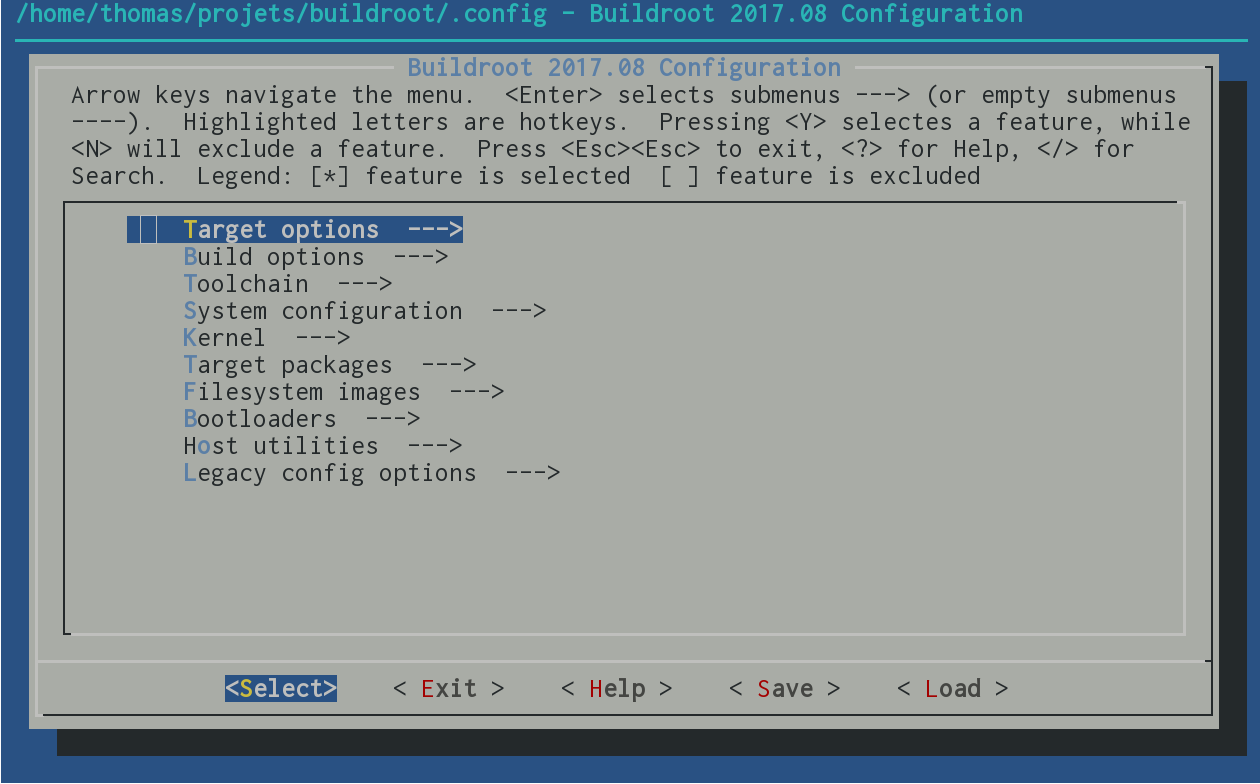
\includegraphics[height=0.8\textheight]{pictures/menuconfig.png}
  \end{center}
\end{frame}

\begin{frame}[fragile]{Lancer une compilation}
  \begin{itemize}
  \item Aussi simple que:
    \begin{block}{}
\begin{verbatim}
$ make
\end{verbatim}
    \end{block}
  \item Si veut garder un log de la compilation pour analyse ou investigation:
    \begin{block}{}
\begin{verbatim}
$ make 2>&1 | tee build.log
\end{verbatim}
    \end{block}
  \end{itemize}
\end{frame}

\begin{frame}{Résultats de compilation}
  \begin{itemize}
  \item Localisé dans \code{output/images}
  \item Selon la configuration, le répertoire contiendra:
    \begin{itemize}
    \item Une ou plusieurs images de root filesystemdans des formats différents
    \item Une image kernel, un ou plusieurs Device Tree blobs
    \item Une ou plusieurs images de bootloader
    \end{itemize}
  \item Pas de standard pourinstaller les images sur une carte
    \begin{itemize}
    \item Trop spécifiques à la carte
    \item Buildroot fournit des outils pour générer une image de carte SD / clef USB
      ({\em genimage}) ou de flasher directement sur certaines plateformes :
      SAM-BA pour Microchip, imx-usb-loader pour i.MX6, OpenOCD, etc.
    \end{itemize}
  \end{itemize}
\end{frame}
